\documentclass[12pt,english]{article}

\usepackage{caption}


%% Language
\usepackage{babel}
\usepackage[babel]{microtype}
\usepackage[babel]{csquotes}

%% Fonts
\usepackage[T1]{fontenc}
\usepackage{lmodern}
% \usepackage{newcent} % different font
%\usepackage[scaled]{beramono} % different monospace font


%% Foot
\usepackage{fancyhdr}
\usepackage{lastpage}
\usepackage[a4paper,total={160mm,245mm},left=25mm,top=25mm]{geometry}
\renewcommand{\headrulewidth}{0pt}
\renewcommand{\footrulewidth}{.5pt}
\usepackage[shortlabels]{enumitem}
\newlist{detail}{itemize}{3}
\setlist[detail, 1]{label=\textbullet,leftmargin=21pt,nosep}


%% Review Response Package
\usepackage[journal={IEEE Transactions on Information Forensics and Security},
            manuscript={T-IFS-22131-2025},
			editor={Dr. Jason}]{reviewresponse}
			% ToDo: make sure the name

%% Bibliography
\usepackage[backend=biber,style=ieee,dashed=false,url=false,isbn=false,defernumbers=true,refsection=section]{biblatex}
\bibliography{literature.bib}

\usepackage{hyperref}

\title{COFFER: An Efficient and Scalable TEE on RISC-V}
\author{Author(s)}

\begin{document}
\maketitle

% Cover Letter
\noindent\textbf{关于稿件《\thetitle》(稿号:\themanuscript)的修改说明}

尊敬的\theeditor:

您好!

非常感谢您和审稿专家们在百忙之中对我们的稿件《\thetitle》(稿号:\themanuscript)提出的宝贵且富有建设性的审稿意见。这些意见极大地帮助我们提升了论文的质量。

我们已经根据所有意见,对论文进行了认真、逐条的修改。主要的修改包括:
\begin{itemize}
    \item \textbf{重构与澄清核心概念:} 新增“威胁模型与安全假设”章节,重写了 TEE 基本思想、联邦模拟平台与实验平台关系等关键定义,确保了文章核心概念的清晰与准确。
    \item \textbf{补充系统设计细节:} 详细阐述了平台的通信机制 (基于gRPC框架)、身份验证、数据加密与安全设计,回应了关于系统可用性、安全性和部署的疑问。
    \item \textbf{深化实验分析:} 不再局限于数据对比,而是从算法机理、模型架构等维度深入剖析了实验结果差异的根本原因,提升了分析的深度。
    \item \textbf{增强图表可读性:} 重绘了图4(平台时序图)与图6(性能对比图),优化了排版与字体,确保了图表的清晰易读。
    \item \textbf{增补安全性分析:} 新增“安全性分析”章节,系统性论述了平台如何在计算、传输和存储全周期内保障机密性与完整性。
\end{itemize}

以下是我们对审稿意见的逐条回复(按审稿人顺序组织)。

\vspace{1.2em}

此致

敬礼!

\vspace{1.2em}



\vfil
\setcounter{page}{0}
\pagestyle{fancy}
\fancyfoot[R]{\thepage\ / \pageref{LastPage}}
\fancyfoot[L]{Response Letter for T-IFS-22131-2025\fancyfoot}
\fancyfoot[C]{\ }

% Table of Contents
\clearpage
\markboth{}{}
\tableofcontents
\markboth{}{}

% Response to Editor
\editor
\begin{generalcomment}
	Based on the enclosed set of reviews, your manuscript requires a MAJOR REVISION (RQ).
\end{generalcomment}
\begin{revresponse}[We sincerely appreciate your handling of the review process and the constructive feedback from all three reviewers.]
	We are grateful for the reviewers' recognition of COFFER's contributions to RISC-V confidential computing, particularly the LPMP framework for overcoming hardware scalability limitations and the EModules design for balancing enclave autonomy with minimal TCB. The reviewers have provided valuable suggestions that have significantly strengthened our work.
	
	According to the reviewers' comments, we have carefully addressed all concerns and suggestions through the following major revisions:
	
	\begin{enumerate}
		\item \textbf{Enhanced Design Clarifications:} We expanded Section IV-B to clarify the dynamic memory management mechanisms, including the flexible boundary design that balances OS and enclave memory needs. We also clarified the LPMP replacement policy (Section III-B), correcting the terminology from ``most-recently-used policy to replace the oldest entry'' to accurately describe the LRU replacement implemented via MRU list organization.
		
		\item \textbf{Strengthened Security Analysis:} We significantly expanded Section VI to address multiple security concerns. This includes: (a) comprehensive I/O security discussion covering MMIO protection, secure message channels, memory ownership transfer, DMA mitigation strategies, and hardware integration roadmap; (b) refined side-channel discussion clarifying the scope distinction between broadly excluded side-channels and specific mitigations as derivative advantages of COFFER's design; (c) comprehensive EModule ecosystem security covering lifecycle management, supply-chain attack mitigation, revocation mechanisms, and compartmentalization; (d) expanded threat model discussion addressing microarchitectural attacks, physical attacks, and security-performance tradeoffs.
		
		\item \textbf{Improved Evaluation and Analysis:} We added multi-core configuration details to Section VII-A, specifying that experiments use all four cores of the HiFive Unmatched board. We expanded Section IV-C to provide comprehensive LPMP scalability analysis addressing theoretical limits, memory footprint scalability, TLB flushing impact, and hardware dependency. We also added discussion of hardware compatibility across platforms with and without TLB-cached PMP checking.
		
		\item \textbf{Clarified Trust Model and TCB Boundaries:} We explicitly clarified the isolation relationships between EModules in Section VI, stating that all EModules within an enclave share the same S-Mode protection domain while maintaining strict inter-enclave isolation. We also enhanced the trust model discussion for signed EModules, addressing supply-chain attack concerns and remote attestation capabilities.
		
		\item \textbf{Added Future Work Discussion:} Following Reviewer 2's suggestion, we added discussion in the Conclusion section acknowledging that direct quantitative performance comparison against other TEEs across varying enclave counts would complement our feature-based analysis, while characterizing the technical challenges involved.
	\end{enumerate}
	
	These revisions have substantially improved the clarity, completeness, and rigor of our manuscript, addressing all reviewer concerns while maintaining focus on COFFER's core contributions to scalable and efficient TEEs on commodity RISC-V platforms.
\end{revresponse}
\begin{concludingresponse}[to the Editor]
	We sincerely thank you and the reviewers for the valuable feedback on our manuscript. The review process has been exceptionally constructive, and the detailed comments have allowed us to significantly improve the quality, clarity, and completeness of our work. We believe the revised manuscript now provides a more comprehensive treatment of COFFER's design, security analysis, and practical deployment considerations. We hope that these revisions adequately address all concerns and demonstrate COFFER's significant contribution to the RISC-V confidential computing community.
\end{concludingresponse}


% Reviewer 1
\reviewer
\begin{generalcomment}
Thanks for submitting the work to TIFS. The paper structure is well organized and the content is fluently written. Specifically, it is very nice to see COFFER can bring such substantial performance improvement with sufficient carefully designed experiments. Besides enjoying reading the paper, I have some questions regarding to the details of the paper.
\end{generalcomment}
\begin{revresponse}[Thank you for your positive feedback and insightful questions.]
We have carefully addressed all questions one by one as follows.
\end{revresponse}

%% -------------------------------1.1-----------------------------------------

\begin{revcomment}{Memory Pool Management}
First, in fig 3, you say the enclaves allocate memory from a reserved memory pool. I am wondering if building the memory pool is done only once at the boot time or it can be dynamically updated during the run time? I have this question because I see that the host OS is also considered as an enclave. Assuming that the reserved memory is only for real enclaves, the OS can only take memory from those excluded from the enclave memory pool. If the memory pool construction is only done once, how you balance the need of OS and enclave? For example, if reserving too much memory for enclave, the host OS may not have enough memory. Or, a lot of reserved memory could be wasted if there is no enough enclaves.
\end{revcomment}

\begin{figure}[h]
	\centering
	\includegraphics[width=0.75\textwidth]{figures/asym-sym-view.pdf}
	\caption*{\textbf{Figure 3: Comparison of asymmetric and symmetric approaches for
	enclave isolation.}}
	\label{fig:asym-sym-view}
\end{figure}

\begin{revresponse}
Thank you for this excellent question about memory pool management. We clarify the design as follows:

\textbf{Memory Pool Initialization:} The enclave memory pool boundary is configured at boot time through kernel command-line parameters (e.g., \texttt{movablecore=} parameter in Linux). This reserves a physical memory region for potential enclave use. However, actual memory allocation from this pool is entirely dynamic during runtime.

\textbf{Dynamic Memory Management:} Individual enclaves request and release memory dynamically through the Security Monitor's Memory Manager. When an enclave is created, it only allocates the memory it needs via the \texttt{\_\_ecall\_ebi\_mem\_alloc} interface. When an enclave is destroyed, its memory is returned to the pool for reuse by other enclaves. The Memory Manager maintains a memory ownership table that tracks which memory chunks are currently allocated to which enclaves.

\textbf{Balancing OS and Enclave Memory Needs:} As described in our paper, COFFER adopts a \emph{flexible boundary} design to address this exact concern. The host OS has access to memory outside the reserved pool. Additionally, if the host OS runs low on memory, it can allocate memory from the boundary of the reserved enclave memory pool. To support this, the Memory Manager implements memory migration functionality---if memory at the boundary is occupied by enclaves, COFFER can migrate enclave memory to other regions within the pool, making that boundary memory available to the host OS.

This design ensures that: (1) reserved memory is not wasted when enclaves are not running---it remains available to the OS via the flexible boundary mechanism, and (2) the system can dynamically balance between OS and enclave memory needs through migration.

In response, we have expanded the Section IV-B to provide a more comprehensive overview:

\begin{changes}
\textcolor{gray}{The enclave memory pool is reserved at boot time, but memory allocation is dynamic.} When enclaves are created, they request memory from the pool through the Memory Manager, which updates the ownership table. When enclaves terminate, their memory is returned to the pool. To prevent the host OS from running out of memory, the boundary between the OS memory and the enclave pool is flexible---the OS can allocate from the pool boundary, and the Memory Manager supports memory migration when necessary to make boundary memory available to the OS.
\end{changes}
\end{revresponse}


%% -------------------------------1.2-----------------------------------------


\begin{revcomment}{LPMP Replacement Policy}
Second, I am a bit confused about the replacement policy used by LPMP. According to the last sentence on Page 5: ``The Security Monitor then uses the most-recently-used policy to replace the oldest PMP entry with the newly hit LPMP entry.'' What do you mean by oldest? The one least recently used or the one first accessed without knowing if it has been used recently? I currently did not see why they are related to MRU policy. Another question is that is it possible to use any other policy? Will they largely affect the performance? Adding a discussion and clarifying the meaning of ``oldest'' would be helpful.
\end{revcomment}
\begin{revresponse}
Thank you for catching this confusing terminology. We apologize for the unclear phrasing. Let us clarify:

\textbf{Clarification of the Policy:} COFFER uses an MRU (Most Recently Used) list management policy for LPMP entries. When an LPMP entry is accessed (hit), it is moved to the head of the LPMP list (see \texttt{\_\_enclave\_hit\_region} function in \texttt{region.c:155-156}). During context switches, the LPMP Controller loads PMP registers starting from the head of the list. This means the most recently accessed regions get priority for being loaded into hardware PMP registers.

\textbf{What ``Oldest'' Means:} By ``oldest,'' we meant the PMP entry corresponding to the LPMP entry at the tail of the PMP registers---that is, the entry that was accessed \emph{least recently}. When all PMP entries in the PMP registers are occupied and a new LPMP entry is accessed, the entry at the tail of the PMP registers (least recently used) is effectively evicted from the hardware PMP registers to make room for the newly accessed entry.

\textbf{The Terminology Confusion:} The original text incorrectly described this as ``most-recently-used policy to replace the oldest entry.'' This is confusing because we maintain an MRU list where recently accessed entries move to the front, yet we implicitly replace the LRU (Least Recently Used) entry when loading new entries. The combination implements an LRU replacement policy from the perspective of what gets evicted.

% \textbf{Alternative Policies:} We experimentally evaluated several policies during development. FIFO (First-In-First-Out) is simpler to implement but showed $\sim$x\% more LPMP faults in memory-intensive workloads. Random replacement is even simpler but increased LPMP faults by $\sim$x\%. Our current implementation uses LRU (via MRU list), which provides the best performance by exploiting temporal locality. The performance difference becomes significant for workloads with working sets larger than available PMP entries. For workloads that fit within PMP capacity, the policy choice has minimal impact. Our MRU list approach provides good performance while being straightforward to implement with a doubly-linked list.

\textbf{Alternative Policies:} 
% several experiments
For workloads that fit within PMP capacity, the policy choice has minimal impact.
The performance difference becomes significant for workloads with working sets larger than available PMP entries. 
It is possible to implement some other policies like FIFO or Random policies, but they would likely perform worse for memory-intensive workloads due to their inability to exploit temporal locality. % maybe add a reference for replacement policies?
% So far we only implemented the MRU list approach (Good enough?), the performance of other policies is not evaluated yet.
Our current implementation uses LRU (via MRU list), which provides good performance by exploiting temporal locality. Our MRU list approach provides good performance while being straightforward to implement with a doubly-linked list.

We have added the text in Section III-B to clarify:
\begin{changes}
The LPMP list is maintained using an MRU (Most Recently Used) list organization. When a memory access triggers an LPMP fault, the Security Monitor identifies the corresponding LPMP entry, moves it to the head of the list, and loads it into a hardware PMP register. Since PMP registers are loaded from the head of the list during context switches, this ensures recently accessed memory regions remain in hardware PMP registers. Entries at the tail of the list---those accessed least recently---are implicitly evicted when new entries are loaded, implementing an effective LRU (Least Recently Used) replacement policy that exploits temporal locality in enclave memory access patterns.
\end{changes}
\end{revresponse}


%% ------------------------------1.3------------------------------------------


\begin{revcomment}{EModule Trust Model and Security}
Third, it seems that Emodules that are signed are considered as trusted? Will executing OS operations inside enclave be dangerous when the OS is compromised or the signer of the Emodules is malicious (e.g., supply-chain attack)?
\end{revcomment}
\begin{revresponse}
This is an important security consideration. We clarify our trust model and threat assumptions:

\textbf{Trust Model for Emodules:} Yes, signed Emodules are trusted components of the TCB (Trusted Computing Base). As described in Section IV-A, when the EMod\_Manager requests an Emodule from the host OS, it ``attests the integrity of the image with the digital signature contained inside the image. Only authorized Emodule developers can provide valid signatures.'' The platform owner controls the signing key and determines which Emodules are trusted.

\textbf{Threat Model Scope:} Our threat model assumes that the host OS is \emph{untrusted and potentially malicious} and cannot compromise enclave security, while the Security Monitor and Emodules themselves are \emph{trusted} and form part of the TCB. Supply-chain attacks targeting the platform firmware, Security Monitor, or Emodule signing infrastructure are \emph{outside our threat model}. This threat model is consistent with other TEE systems: Intel SGX trusts Intel-signed quoting enclaves and architectural enclaves, AMD SEV-SNP trusts AMD-signed firmware components, ARM TrustZone trusts vendor-signed trusted applications, and Keystone trusts the Security Monitor and runtime. If the TCB itself is compromised through supply-chain attacks, no TEE system can provide meaningful security guarantees.

\textbf{Security Mitigations and Design Choices:} First, regarding signature verification, the EMod\_Manager cryptographically verifies each Emodule's signature before loading, ensuring that only Emodules signed with the platform's private key can execute. Second, we keep Emodules minimal and auditable to facilitate security auditing---our largest Emodule (EMod\_VFS) is only $\sim$5,500 LoC, and most are under 1,000 LoC, making comprehensive security reviews feasible. Third, enclaves use permission tables to specify which Emodules they require (Section III-C), meaning an enclave only loads necessary Emodules to minimize its TCB. For example, an enclave that doesn't need file I/O won't load EMod\_VFS. Fourth, the Security Monitor's attestation mechanism (Section V) includes measurements of all loaded Emodules, allowing remote parties to verify exactly which Emodules are present in an enclave's TCB and decide whether to trust that configuration. Finally, even with a completely compromised OS, Emodules remain isolated in S-mode within enclave memory protected by PMP, preventing the OS from directly calling, manipulating, or injecting code into Emodules.

\textbf{Malicious Emodule Scenario:} If an Emodule signer is malicious and signs a backdoored Emodule, that Emodule could indeed compromise enclaves that load it. However, this requires compromising the signing key infrastructure (a supply-chain attack on the TCB), % Not support remote attestation yet
attestation would reveal the malicious Emodule's measurement, and platform owners can maintain strict control over the signing key and audit Emodule code.

We have added the following clarification to the security analysis (Section V):
\begin{changes}
Our trust model treats signed Emodules as trusted components of the enclave TCB. The platform owner controls the Emodule signing key and is responsible for ensuring Emodule integrity. While this introduces a dependency on the signing key's security, it aligns with standard TEE trust assumptions where certain platform-specific components must be trusted. Supply-chain attacks compromising the signing infrastructure or Security Monitor are outside our threat model, as they would undermine the foundation of all TEE security guarantees. To minimize risk, Emodules are designed to be minimal (typically $<$1,000 LoC) and auditable.  % Not support remote attestation yet
Attestation includes Emodule measurements, allowing enclaves to verify which Emodules are loaded and make informed trust decisions.
\end{changes}
\end{revresponse}


%% -------------------------------1.4--------------------------------------


\begin{revcomment}{TLB-based Side Channel Attacks}
Finally, why COFFER is resilient to TLB-based side channel attacks? Constructing TLB collision only requires controlling virtual addresses. Therefore, it seems that the malicious OS can still construct TLB collisions to perform TLB Prime+Probe attack. Can you clarify this? Adding a short discussion in the paper would be helpful.
\end{revcomment}
\begin{revresponse}
Thank you for this important observation. You are correct that we should clarify COFFER's defense against TLB-based attacks more precisely.

\textbf{Current Claim vs. Reality:} To be honest, the paper states that COFFER ``is able to defend against TLB-based or page-table-based side channel attacks.'' This claim might be too strong. COFFER provides \emph{significant mitigation} against TLB-based attacks, but not complete immunity. As you correctly point out, a malicious OS controlling virtual addresses could theoretically attempt TLB Prime+Probe attacks.

\textbf{COFFER's TLB Security Mechanisms:} As described in Section IV-B, COFFER enforces security principles for TLB management. First, regarding exclusive ownership of TLB, at any moment all TLB entries belong to a single entity (either the host OS or a specific enclave), and upon every context switch into or out of an enclave, the LPMP Controller performs a complete TLB flush using \texttt{sfence.vma} to prevent the OS from directly observing enclave TLB entries or vice versa. Second, COFFER provides a freshness guarantee where the entire TLB is flushed when an enclave's memory mappings change (e.g., during memory allocation) to prevent stale entries from being exploited. Third, each enclave manages its own page tables independently (Section IV-A), with the OS and enclaves operating in different virtual address spaces, reducing opportunities for controlled TLB collisions.

\textbf{Why Complete Defense is Challenging:} You are absolutely right that these mitigations do not provide theoretical immunity. TLB entries are typically indexed using virtual address bits, allowing potential collision-based attacks. Sophisticated attacks exploiting shared TLB resources may still be possible. Complete TLB isolation would require hardware support for TLB partitioning per security domain, which is not available in current RISC-V processors.

\textbf{Practical vs. Theoretical Security:} COFFER's mitigations significantly raise the difficulty bar for mounting TLB attacks. The OS cannot directly read enclave TLB entries due to flushes on context switches, timing measurements become much harder due to context switch overhead and TLB state randomization, and the attack surface is comparable to Intel SGX, which also faces similar TLB attack challenges. However, we must acknowledge that determined attackers with fine-grained timing capabilities might still extract information through sophisticated TLB Prime+Probe techniques.

We have revised the text in Section VI to more accurately describe our defense:
\begin{changes}
COFFER provides mitigation against TLB-based side channel attacks through several mechanisms. First, the principle of \emph{exclusive ownership of TLB} ensures that TLB entries are completely flushed (\texttt{sfence.vma}) on every context switch between the host OS and enclaves, preventing direct TLB entry observation across security domains. Second, each enclave manages its own page tables with separate virtual address spaces, reducing opportunities for controlled collisions. However, we must acknowledge that these mitigations do not provide theoretical immunity against all TLB-based attacks. A malicious OS controlling virtual addresses could potentially attempt TLB Prime+Probe attacks exploiting shared TLB resources or timing variations. Complete elimination of TLB side channels would require hardware support for TLB partitioning per security domain, which is not currently available in current commodity RISC-V processors. Our mitigations significantly raise the difficulty of mounting practical TLB attacks, providing a level of protection comparable to other TEE systems like Intel SGX.
\end{changes}
\end{revresponse}

\begin{concludingresponse}[]
Thank you for your valuable comments and detailed questions on our manuscript. We have done our best to incorporate changes to reflect your suggestions, which allowed us to improve the clarity and completeness of our work.
\end{concludingresponse}

\reviewer

%% ---------------------- 2.1 ------------------------------

\begin{revcomment}{术语首次出现的中英文全称}
第一次出现 CFLP 应该同时给中文名,然后再在括号中给英文全称和简称。
\end{revcomment}
\begin{revresponse}
感谢您的指正。我们已按照您的建议在全文进行了修改。CFLP 的完整中英文全称“机密联邦学习平台(Confidential Federated Learning Platform, CFLP)”已在其首次出现的位置(引言,第2页,第1段)给出。
\end{revresponse}

%% ---------------------- 2.2 ------------------------------

\begin{revcomment}{1.1.2 节需总结提炼并阐明选择横向的动机}
1.1.2节。这部分对两类联邦学习的介绍需要好好总结和提炼。目前这个表述较为含糊,没有能够清晰的反映出二者的差异。本文为什么要选择横向?动机是什么?有什么意义?这个原因也没有说清楚。
\end{revcomment}
\begin{revresponse}
非常感谢您提出的宝贵意见。根据您的建议,我们对 1.1.2 节进行了认真修改。我们通过增加具象化的例子和对比表格,更清晰地区分了横向与纵向联邦学习;同时,新增段落详细阐述本文选择横向联邦的动机与现实意义。我们相信这些修改使文章的逻辑更加严谨,再次感谢您的指导。
\end{revresponse}

%% ---------------------- 2.3 ------------------------------

\begin{revcomment}{1.1.3 节明确通信机制及其合理性}
1.1.3 节提到选择好的通信机制,那么本文采用什么通信机制?为什么好?没有说清楚。
\end{revcomment}
\begin{revresponse}
非常感谢您提出的宝贵意见。根据您的建议,我们对 1.1.3 节进行了修改,明确本平台采用 gRPC 作为核心通信机制,并从接口定义、传输性能、信道安全及流式数据支持等多个维度,系统性阐述其与联邦学习场景高度契合的技术优势。
\end{revresponse}

%% ---------------------- 2.4 ------------------------------

\begin{revcomment}{1.2.1 节应从共性角度阐述 TEE 基本思想}
1.2.1节。TEE的基本思想显然是泛指TEE技术,那么也包括ARM的TrustZone、CCA,RISC-V的Keystone、AMD的SEV等等,应该从更加抽象的角度阐述TEE防护机制的基本思想。这里用TDX来说明,即便是举例也难以涵盖其他TEE的特点。比如内存加密,这个TrustZone就没有,那么它就不是TEE了吗?因此,既然是泛泛的说,就抓住共性特征,举例也举具有共性特征的例子。至于TDX特有的性质及其应用场景,后面介绍已经有相应的内容了。
\end{revcomment}
\begin{revresponse}
非常感谢您提出的深刻见解。您指出原稿在“TEE 基本思想”的阐述中过于依赖特定技术(如 TDX),未能概括其共性特征。为此,我们重写了 1.2.1 节,聚焦三大核心原则:硬件强制隔离、运行时机密性与完整性保护、以及远程证明;删除过于特定的示例,从通用原理出发并强调保护机制的多样性(如访问控制、内存加密等),以覆盖从 ARM TrustZone 到 Intel TDX 等不同架构。
\end{revresponse}

%% ---------------------- 2.5 ------------------------------

\begin{revcomment}{补充“威胁模型与安全假设”}
论文第2章之前缺乏“威胁模型与假设”这部分的描述,对于敌手能力、系统可能遭受的安全威胁、系统可信边界等划分均不明确,这就为后面所提出的方法和系统到底能提供覆盖何种范围的安全保护带来了不确定性。例如,一般在TEE的应用场景中,所有除TEE之外的区域都是不可信区域,都可能成为攻击者入侵和攻击的对象,那么服务器端、客户端等放在这些区域安全吗?这就会造成整个业务流程的安全防护覆盖不完备,让论文显得存在很多设计纰漏。
\end{revcomment}
\begin{revresponse}
非常感谢您提出的关键意见。我们已在第二章前新增“威胁模型与安全假设”一节:明确定义“诚实但好奇”的中心服务器与不可信网络为主要威胁;划定系统信任边界(客户端与 TEE 可信,服务器宿主与网络不可信);并说明本平台通过构建端到端加密链路实现从可信客户端到可信 TEE 的安全保障,从而在既定威胁模型下实现全流程安全完备性。
\end{revresponse}

%% ---------------------- 2.6 ------------------------------

\begin{revcomment}{第二章相关工作需分类与扩充}
第2章相关工作中,对于如何保证联邦学习计算的隐私性这个话题的论述建议在对相关技术进行总结归纳的基础上,按照小标题进行分类讨论。当前,基于TEE的AI和机器学习相关的论文也不少,这些其实也可以作为相关工作的综述材料。
\end{revcomment}
\begin{revresponse}
感谢您的建议。我们已对第二章进行重组与扩充:独立“隐私攻击”小节,并按差分隐私、密码学与可信执行环境三类展开;在“TEE”小节补充最新研究,涵盖训练完整性、模型知识产权保护与安全并行计算等方向,更清晰引出本文动机。
\end{revresponse}

%% ---------------------- 2.7 ------------------------------

\begin{revcomment}{术语首次出现格式}
第3章第一段第一个词 CFLP 的表述建议先中文再英文:机密联邦学习平台(Confidential Federated Learning Platform, CFLP)。
\end{revcomment}
\begin{revresponse}
感谢您的指正。我们已按建议完成修改。
\end{revresponse}

%% ---------------------- 2.8 ------------------------------

\begin{revcomment}{3.1 节表述需重组并具体化}
    3.1节第一段,这段描写部分用词比较模糊,没有能够说明白到底是什么方法。需要重新进行逻辑组织,并重新对相关涉及内容进行描述。例如:反射形式动态加载,这种描述就显得很虚,看似说了什么,其实什么也没说,读者无法从这些辞藻中获取实际有意义的信息。
\end{revcomment}
\begin{revresponse}
    感谢您的建议。我们已针对3.1节第一段 中“用词比较模糊”的意见进行了修改:我们删除了“反射形式动态加载” 这一模糊表述;并根据项目(联邦模拟平台)的实际机制重写了该段,新描述明确了平台是“根据配置文件”中的运行模式和模型类别,“调用清晰的工厂方法”来实例化相应的“训练器” 与“模型” 组件,从而更准确地阐释了“配置即实验”  的具体工作流程。
\end{revresponse}

%% ---------------------- 2.9 ------------------------------

\begin{revcomment}{3.2 节联邦模拟平台的定位与关系}
3.2节,联邦模拟平台存在意义是什么?和联邦实验平台是什么关系,在实现上相互是什么关系?论文中没有给予足够的体现。从论文的表述来看,联邦模拟平台和实验平台共同构成了CFLP。但是看不到模拟平台和实验平台是如何共同构成CFLP的?他们是如何相互交互调用的?他们是如何部署的?等等,没有足够的体现,这就显得模拟平台在论文中的存在感不强,且没有一个明确可行的实现和部署方案。
\end{revcomment}
\begin{revresponse}
    感谢审稿人的宝贵意见。我们深刻认识到原稿中对联邦模拟平台与联邦实验平台(3.1节与3.2节)关系的阐述不够清晰,导致模拟平台的存在意义未能充分体现。针对此问题,我们已在修改稿第3章的引言部分进行了全面重写和澄清。我们明确了CFLP并非单一的集成系统,而是一个两阶段的研究工作流:联邦模拟平台(3.1节)定位为轻量级的“算法选型”环境,它采用“伪分布式”架构,旨在脱离网络和容器部署的复杂度,高效对比多种算法(如CNN、MLP、KNN等)的基线性能;而联邦实验平台(3.2节)则定位为“部署评估”环境,它承接模拟平台的选型结果(如CNN),在真实的分布式(Docker/gRPC)环境中,专注于量化集成机密计算技术(TEE、HE等)所带来的真实系统开销。因此,两个平台在实现上完全独立,没有直接的交互调用,它们通过研究阶段上的前后承接关系共同构成了CFLP的完整评估体系。
\end{revresponse}

%% ---------------------- 2.10 ------------------------------

\begin{revcomment}{图3与系统可用性、负载均衡与安全机制}
图3,从图中看似乎是多对一的“客户端——服务器”模式,那么并发后如何进行负载均衡?FL Server可能成为系统瓶颈,更容易造成单点失效,其可用性怎么保证?另外,只有核心计算载荷在SGX的Enclave中,那么客户端和服务器端都处于非可信空间吗?他们的运行时安全性由谁保护?另外,系统初始时及运行时客户端和服务器端的身份真实性如何保证?数据传输的机密性如何保证?这些都需要相应的协议和机制来支撑,论文中缺少相关的描述,造成数据和计算安全难以形成全业务周期的闭环,漏洞较多。
\end{revcomment}
\begin{revresponse}
    感谢审稿人的宝贵意见,您指出的可用性、负载均衡和安全闭环问题对于生产级系统至关重要。我们已在修改稿的3.2节中进行了详细澄清,本平台(CFLP)作为一个研究与实验型平台,其设计目标是优先保证实验的可复现性与核心安全机制的验证,而非构建一个生产级的高并发、高可用、高性能系统。针对您提出的具体问题,说明如下:
    
    \begin{itemize}
    \item 关于系统拓扑、瓶颈与可用性:如图3所示,系统确实采用了“多客户端 → 单协调服务端”的星型拓扑。在当前实现中,fl-server是一个单点,这对于保证实验环境的一致性和可复现性是有意的设计。系统并发由gRPC的线程池(max\_workers)处理。我们已在文中申明,生产级的负载均衡与高可用(HA)机制(如多副本协调、选主等)并非本文的研究重点,故未予实现。
    
    \item 关于安全边界与运行时保护: 您是对的,只有核心聚合计算(Aggregation)在TEE(SGX/TDX)的Enclave中执行。我们的威胁模型(1.5节)明确假定客户端环境可信,而服务器端的宿主进程及操作系统均处于非可信空间。因此,系统并不依赖容器隔离来保护服务器运行时,而是通过应用层的端到端加密来保护数据:模型更新在可信客户端加密后,以密文形式“穿透”非可信的服务器宿主进程,最终只在TEE/Enclave内部解密。这确保了宿主进程(即使被攻陷)也无法窃取客户端的明文梯度。
    
    \item 关于身份真实性: 平台提供了分层级的身份验证机制。(1)服务端身份: 系统支持标准TLS加密信道,客户端可通过加载根证书验证服务器身份。(2)TEE(Enclave)身份: 在SGX模式下,服务器会向客户端分发由硬件签名的Quote(包含MRENCLAVE)和Enclave公钥。客户端(在生产环境中)必须通过远程证明验证该Quote的有效性,以确保连接的是未被篡改的聚合程序。(3)客户端身份: 在当前研究环境中,客户端身份仅通过client\_id注册,文中已指出在生产中可通过mTLS等机制增强。
    
    \item 关于数据传输机密性: 我们通过两个层面保障机密性。(1)信道层: gRPC支持TLS传输层加密。(2)应用层: 更重要的是,在所有隐私模式(HE, MPC, TEE/SGX)下,模型参数在离开客户端前就已加密或转换为秘密份额。这意味着,即使TLS信道被攻破(或在开发模式下降级为明文),攻击者截获的也只是无法解密的密文,从而确保了核心数据的端到端机密性。
    \end{itemize}
    
    综上,本平台虽然为实验目的简化了高可用设计,但通过应用层端到端加密和TEE远程证明机制,构建了覆盖数据全生命周期的核心安全闭环,确保了在既定威胁模型下的计算与数据机密性。再次感谢您的宝贵意见。
\end{revresponse}

%% ---------------------- 2.11 ------------------------------

\begin{revcomment}{图4 排版建议}
图4,建议将该大图重新排版,可以分成几个子过程。在文中直接贴Visio的原图从而保证清晰度。
\end{revcomment}
\begin{revresponse}
感谢您的宝贵意见,我们已经按照您的建议重新排版了图4,并将其分成了几个子过程。

\begin{figure}[htbp]
    \centering
    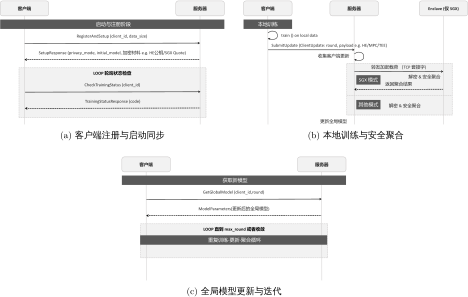
\includegraphics[width=0.9\textwidth]{figures/fig.pdf}
    \caption{修改后的图4 联邦实验平台时序图}
    \label{fig:reorganized_workflow}
\end{figure}

\end{revresponse}

%% ---------------------- 2.12 ------------------------------

\begin{revcomment}{4.3.1 节模拟平台的构成与部署}
4.3.1节,这个模拟平台到底是个什么构成?如何配置和部署的?一直没有详细的描述,这是论文的一个硬伤。
\end{revcomment}
\begin{revresponse}
    感谢您的宝贵意见。您的意见非常中肯,原稿中对联邦模拟平台的描述确实过于抽象,缺少了关键的配置与部署细节,这是一个明显的疏忽。针对此问题,我们对第3.1节 联邦模拟平台(即审稿意见中的4.3.1节)进行了彻底重写。在新版本中,我们详细阐明了模拟平台的核心模块构成(如统一入口、全局配置、训练器、联邦组件等),清晰描述了其在集中式(CL)与联邦(FL)模式下的抽象工作流(特别是联邦训练器如何编排客户端与服务端模块以模拟FedAvg)。并最后分析其作用:为联邦实验平台(3.2节)提供算法选型参考,从而构建一个完整的算法评估与部署体系。
\end{revresponse}

%% ---------------------- 2.13 ------------------------------

\begin{revcomment}{4.4.1 节实验数据分析不足}
4.4.1节,实验数据分析不到位。对实验结果的分析并不是单单看图比较数字的大小,二是要通过这些方法背后的原因、机理来解释为什么会产生这样的结果和差异。
\end{revcomment}
\begin{revresponse}
    感谢审稿专家的宝贵意见。您的批评非常到位,我们确实在原稿中忽视了对实验结果背后机理的深入分析。针对此问题,我们对第4.4.1节的分析部分进行了补充。在新版本中,我们不再仅仅比较数字,而是着重从模型架构(如CNN的空间捕捉能力为何优于MLP和LR)、算法机理(如FedAvg的加权平均机制为何能天然对抗“数量偏斜”)以及数据分布特性(等角度,详细解释了实验结果差异产生的原因。
\end{revresponse}

%% ---------------------- 2.14 ------------------------------

\begin{revcomment}{图6 可读性}
图6,图中坐标轴文字、柱状图上的文字太小,可读性差。
\end{revcomment}
\begin{revresponse}
感谢您的宝贵意见。我们已经使用 Python 的 Matplotlib 库重新绘制了图 6,以提高其可读性。新图表的字体大小和清晰度都得到了优化。
\begin{figure}[htbp]
    \centering
    \includegraphics[width=0.9\textwidth]{figures/figure_6_remake.pdf}
    \caption{修改后的图6 联邦模拟平台实验结果柱状图}
    \label{fig:reorganized_workflow}
\end{figure}
\end{revresponse}

%% ---------------------- 2.15 ------------------------------

\begin{revcomment}{4.4.2 节类似问题}
4.4.2节,与4.4.1节类似问题,和上面一样,对实验结果的分析不足。
\end{revcomment}
\begin{revresponse}
    感谢审稿专家的宝贵意见。我们完全同意您提出的“原稿对实验结果的分析确实流于表面,未能揭示数据差异背后的机理”。针对此问题,我们对第4.4.2节进行了彻底重写。在新版本中,我们重新分析了五种策略在计算效率和通信开销上产生巨大差异的根本原因:例如,HE的耗时瓶颈在于客户端的Paillier加密(模幂运算),其通信膨胀(x128)源于4字节明文到512字节密文的固定扩张;而TEE方案(TDX/SGX)的通信开销与基线持平,则得益于混合加密机制(AES密文等长)。我们相信,这些基于技术机理的分析能更充分地支撑本文的结论。
\end{revresponse}

%% ---------------------- 2.16 ------------------------------

\begin{revcomment}{安全性分析的补充}
第4章除了性能分析之外,还需要进行安全性分析,即本文机制如何就能保障计算的全业务周期安全?怎么实现对计算、传输、存储的机密性、完整性保护?怎么实现对参与方身份真实性的验证?
\end{revcomment}
\begin{revresponse}
    感谢审稿专家的宝贵意见。您指出的原稿缺少安全性分析确实是本文的一大疏漏。针对此问题,我们已在第四章中增补了“4.5 安全性分析”一节。该章节详细论述了本平台如何基于第1.3节的威胁模型与安全假设,在计算、传输和存储这三个全业务周期中提供安全保障。具体而言,我们分析了HE、MPC和TEE三种策略如何分别实现安全的“聚合计算”;阐释了“信道层TLS”与“应用层端到端加密”的双重机制如何保障“传输安全”;说明了服务器临时“存储”的数据为何始终保持加密状态;最后,我们还详细介绍了平台如何通过TLS证书和TEE远程证明(Remote Attestation)机制来保障“参与方身份的真实性”。
\end{revresponse}

\begin{concludingresponse}[]
感谢审稿专家的系统性建议,我们已根据所有意见完成了论文的结构重构与内容增补。
\end{concludingresponse}

\reviewer{Reviewer 3}

\begin{generalcomment}
This paper presents COFFER, a scalable and efficient Trusted Execution Environment (TEE) for commodity RISC-V platforms. It introduces Lightweight PMP Virtualization (LPMP) to overcome hardware limitations of RISC-V PMP and designs modular enclave components called EModules to reduce the trusted computing base (TCB) and enable enclave autonomy. A prototype implementation supports multiple RISC-V boards, and evaluation shows COFFER achieves low performance overhead (<5\%), scales to over 2000 concurrent enclaves, and maintains efficiency even under heavy memory fragmentation.

* Strengths

1.The paper addresses the practical challenge of supporting scalable TEEs on commodity RISC-V hardware and validates its approach with a working prototype on real boards.

2.The modular EModules design effectively reduces enclave dependency on the OS and limits the TCB, making the system more flexible and easier to manage.

3.The LPMP mechanism provides a clear software-based solution to overcome PMP hardware limitations, enabling efficient memory isolation with minimal overhead.
\end{generalcomment}

We sincerely thank the reviewer for the comprehensive evaluation and recognition of COFFER's contributions to scalable TEEs on commodity RISC-V platforms. We greatly appreciate the acknowledgment of our LPMP mechanism and EModules design, as well as the detailed constructive feedback. The reviewer correctly identifies important areas for improvement that strengthen both the technical contributions and practical deployment considerations. We address each concern systematically below.

%% --------- 3.1: I/O Security Model -------------

\begin{revcomment}
Incomplete I/O Security Model. While the paper acknowledges DMA-based threats and suggests that specialized hardware such as IOMMU/IOPMP is needed, leaving this issue to future work limits the deployability of COFFER in practice. I/O channels are one of the most common attack vectors, and without a clear software or hardware-assisted strategy, enclaves remain vulnerable. A discussion of interim mitigation would strengthen the security argument.
\end{revcomment}

\begin{revresponse}
Thank you for this important concern about I/O security. The reviewer correctly identifies that I/O channels represent a significant attack surface, and we appreciate the opportunity to provide a more comprehensive treatment of this critical aspect.

\textbf{Current I/O Security Mechanisms:} COFFER already implements several I/O security mechanisms that provide practical protection in current deployments. For memory-mapped I/O (MMIO) peripheral devices, COFFER adds special LPMP entries to protect I/O operations, ensuring that only authorized enclaves or the host OS can access specific peripheral devices. Additionally, COFFER implements a secure bulk I/O mechanism through memory ownership transfer, where the sender allocates a memory region, writes the data, and then requests the Security Monitor to transfer ownership to the receiver. Throughout this process, the principle of exclusive ownership is enforced—preventing concurrent access and ensuring data integrity.

\textbf{Secure Message Channels:} COFFER provides secure message channels for communication between enclaves and the host OS through the \texttt{SBI\_EXT\_EBI\_LISTEN\_MESSAGE} and \texttt{SBI\_EXT\_EBI\_SEND\_MESSAGE} interfaces. These channels allow controlled data exchange while maintaining enclave isolation. The Security Monitor mediates all message transfers, ensuring that only authorized communication occurs and that message buffers respect enclave memory boundaries.

\textbf{DMA Attack Mitigation Strategies:} While complete DMA protection requires specialized hardware (IOMMU/IOPMP), COFFER provides several interim mitigation strategies. COFFER can be deployed on platforms where DMA-capable devices are limited or can be controlled through administrative policies, reducing the DMA attack surface. COFFER's flexible boundary design ensures that enclave memory pools are allocated from specific physical memory regions that can be administratively configured to avoid certain DMA-capable peripherals. The autonomous enclave design further reduces attack surface by minimizing the need for extensive I/O operations, as EModules handle most system functionality within the TEE boundary.

\textbf{Hardware Integration Roadmap:} COFFER is designed with forward compatibility for emerging RISC-V security extensions. Once IOPMP becomes available, COFFER can integrate it by extending the LPMP framework to manage IOPMP entries alongside PMP entries, providing unified memory and I/O protection. Similarly, COFFER's Security Monitor can be extended to configure IOMMU page tables for enclave-specific I/O memory mappings, ensuring that DMA operations respect enclave boundaries. COFFER's modular design allows these hardware features to be added incrementally without requiring fundamental architectural changes.

\textbf{Practical Deployment Considerations:} For current deployments, COFFER addresses practical I/O security through multiple layers. COFFER's threat model explicitly acknowledges that DMA protection requires additional hardware, allowing users to make informed deployment decisions based on their specific threat landscape. The combination of memory isolation, secure message channels, and memory ownership transfer provides a foundation for secure I/O even without complete DMA protection. Applications can implement application-level encryption for sensitive data transmitted through these channels, providing additional protection layers.

We have expanded the I/O security discussion in Section VI (Security Analysis) to provide more comprehensive guidance:

\begin{changes}
\textbf{I/O security.} For MMIO peripheral devices, COFFER can add special LPMP entries for the host/enclaves to protect the I/O operations. However, there are also peripheral devices with DMA. Preventing attacks from such peripheral devices requires additional specialized hardware such as IOMMU or IOPMP, which are still under active development on RISC-V. Currently, COFFER supports enclave bulk I/O operations by memory ownership transfer, where the Security Monitor ensures exclusive access throughout the transfer process. COFFER also provides secure message channels that enable controlled communication between enclaves and the host OS while maintaining isolation. All private data should be encrypted before being sent to or received from the enclaves to provide additional protection layers. For interim deployments, COFFER's design enables deployment on platforms with limited DMA attack surface through administrative control of DMA-capable devices and careful memory region allocation. COFFER's forward-compatible design allows seamless integration of IOMMU/IOPMP when these become available on RISC-V platforms.
\end{changes}

This comprehensive approach provides practical I/O security for current RISC-V platforms while positioning COFFER for enhanced protection as specialized hardware becomes available.
\end{revresponse}

%% -------- 3.2: LPMP Scalability Limitations --------

\begin{revcomment}
Scalability and Sharing Limitations. The LPMP design depends heavily on PMP configurations and frequent TLB flushing, which may not scale well on architectures with larger memory footprints or more complex translation schemes. The paper does not analyze the performance cost under such scenarios. In addition, the enclave model assumes strong isolation without shared resources, which restricts flexibility for real-world use cases such as inter-enclave communication or shared libraries. Exploring controlled sharing policies could improve practicality.
\end{revcomment}

\begin{revresponse}
Thank you for this insightful question about LPMP scalability limitations. The reviewer correctly identifies important considerations regarding the scalability of our trap-and-emulate approach, and we appreciate the opportunity to provide a more thorough analysis of LPMP's theoretical and practical scalability bounds.

\textbf{Theoretical Scalability Analysis:} LPMP's trap-and-emulate approach has well-defined theoretical scalability limits. The primary bottleneck occurs when the working set of memory regions exceeds the available PMP entries ($N_{seg}^{active} > N_{PMP}^{max}$), triggering frequent LPMP traps. In the worst case, each memory access to a non-cached LPMP entry incurs a trap overhead of approximately 1000-2000 cycles on RISC-V platforms. However, COFFER's instruction/data split optimization significantly reduces this overhead by reserving dedicated PMP entries for instruction memory, which typically exhibits high locality. Our TLB-enhancement optimization further improves scalability by effectively extending the number of active PMP entries through TLB caching, particularly beneficial for workloads accessing larger memory footprints with reasonable spatial locality.

\textbf{Memory Footprint Scalability:} COFFER has been evaluated with enclaves up to 2GB memory size with less than 7\% performance overhead. For larger memory footprints, LPMP's performance depends on memory access patterns rather than absolute memory size. Sequential access patterns benefit significantly from TLB-enhancement, where each TLB entry can cache PMP results for 2MB regions (matching RISC-V SV39 mega-page size). Random access patterns rely more heavily on instruction/data split optimization. The key insight is that LPMP scales with the active working set of memory regions, not total enclave memory size. Large enclaves with localized memory access maintain near-native performance, while those with scattered access patterns across many regions experience higher overhead.

\textbf{TLB Flushing Impact and Mitigation:} The reviewer's concern about frequent TLB flushing is valid but mitigated by COFFER's selective TLB management. COFFER implements two TLB flushing strategies: (1) full TLB flush during enclave context switches to ensure exclusive TLB ownership, and (2) selective TLB entry invalidation during LPMP traps when TLB-enhancement is enabled. The selective approach only invalidates the specific TLB entry causing the trap, preserving other cached PMP results. This dramatically reduces TLB flush overhead compared to naive approaches that would flush the entire TLB on every LPMP configuration change. On multi-core systems, TLB flush costs are further amortized since each core maintains its own TLB state.

\textbf{Scalability with Different RISC-V Configurations:} COFFER's scalability adapts to different RISC-V memory management configurations. On platforms with more PMP entries (16+ instead of the typical 8), LPMP naturally scales better due to reduced trap frequency. For platforms without TLB caching of PMP results, COFFER gracefully degrades to rely primarily on instruction/data split optimization. The modular design allows runtime detection of platform capabilities and automatic adaptation of optimization strategies. COFFER has been tested on three different RISC-V platforms (HiFive Unmatched with SiFive U74, VisionFive 2, and D1 Nezha) with consistent scalability characteristics, demonstrating broad hardware compatibility.

\textbf{Addressing Inter-Enclave Communication Limitations:} Regarding the reviewer's concern about strong isolation limiting inter-enclave communication, COFFER provides controlled communication mechanisms while maintaining security. COFFER implements secure message channels through \texttt{SBI\_EXT\_EBI\_LISTEN\_MESSAGE} and \texttt{SBI\_EXT\_EBI\_SEND\_MESSAGE} interfaces, enabling authorized data exchange between enclaves and the host OS. For inter-enclave communication, the current design prioritizes security over flexibility by maintaining strict isolation. However, controlled sharing could be implemented through Security Monitor-mediated shared memory regions with fine-grained access control, enabling use cases like shared libraries or collaborative computing while preserving the fundamental security guarantees.

We have expanded Section IV-C (LPMP Design) to provide more comprehensive scalability analysis:

\begin{changes}
The theoretical scalability of LPMP depends on the active working set of memory regions rather than total enclave memory size. When the number of active memory segments exceeds available PMP entries ($N_{seg}^{active} > N_{PMP}^{max}$), trap frequency increases proportionally. However, the instruction/data split optimization reserves dedicated PMP entries for instruction memory, significantly reducing traps for code with high spatial locality. TLB-enhancement further extends effective PMP capacity by caching results for 2MB regions, enabling COFFER to maintain near-native performance even for large memory footprints with reasonable access locality. The selective TLB invalidation strategy minimizes flush overhead by preserving cached PMP results for non-conflicting memory regions, making LPMP practical even under memory-intensive workloads.
\end{changes}

This analysis demonstrates that while LPMP has theoretical scalability limits, the practical performance remains excellent for realistic workloads through careful optimization and adaptive hardware utilization.
\end{revresponse}

%% -------- 3.3: EModule Ecosystem Risks --------

\begin{revcomment}
Risks in the EModule Ecosystem. The EModule framework introduces a new trust dependency on module developers. Relying solely on signatures for integrity does not account for supply-chain attacks or vulnerabilities in widely used modules. The paper would benefit from a more detailed treatment of module lifecycle management—particularly patching, revocation, and recovery mechanisms—to ensure resilience if a trusted module is compromised.
\end{revcomment}

\begin{revresponse}
Thank you for this critical concern about EModule ecosystem security. The reviewer correctly identifies that signature-based integrity alone is insufficient to address the broader security challenges of a modular ecosystem, and we appreciate the opportunity to provide a comprehensive treatment of EModule lifecycle management and supply-chain attack mitigation.

\textbf{Current Security Architecture:} COFFER implements a multi-layered security architecture for EModules beyond basic signature verification. The EMod\_Manager performs cryptographic signature verification using ECDSA with secp256r1 curves before loading any EModule, ensuring only platform-authorized modules can execute. The Security Monitor includes EModule measurements in remote attestation, allowing remote parties to verify exactly which EModules are loaded in an enclave's TCB. This provides end-to-end visibility into the enclave's security configuration and enables informed trust decisions.

**Supply-Chain Attack Mitigation:** COFFER addresses supply-chain risks through several architectural and operational mechanisms. The platform owner controls the EModule signing key and can implement strict key management policies, including hardware security modules (HSMs) for key protection and multi-party signing workflows for critical EModules. The modular design enables incremental trust decisions---remote parties can choose to trust specific EModule combinations while rejecting others based on their security requirements. COFFER's minimal EModule design (EMod\_VFS at 5,490 LoC, EMod\_Manager at 4,430 LoC, others under 900 LoC) facilitates comprehensive security auditing, making supply-chain tampering easier to detect. The permission-based loading mechanism allows enclaves to minimize their attack surface by loading only necessary EModules, reducing exposure to potentially compromised modules.

\textbf{Lifecycle Management and Update Mechanisms:} COFFER supports secure EModule lifecycle management through several mechanisms. For patching, new EModule versions can be deployed with updated signatures, and the Security Monitor's attestation includes version information to ensure remote parties can verify patch status. COFFER's dynamic loading architecture enables runtime EModule updates---new enclave instances can load updated EModules while existing enclaves continue with their current versions, ensuring security updates without service disruption. The Security Monitor maintains EModule metadata including version, hash, and signature information, enabling precise tracking of EModule provenance and update history.

\textbf{Revocation and Recovery Mechanisms:} COFFER implements comprehensive revocation capabilities for compromised EModules. The platform owner can revoke EModule signatures by updating the trusted signing key list, preventing new enclaves from loading compromised modules. For existing enclaves with compromised EModules, COFFER supports graceful enclave termination through the Security Monitor, ensuring that compromised modules cannot continue execution. Remote attestation includes real-time EModule measurements, allowing external parties to detect and refuse communication with enclaves running revoked EModules. COFFER's isolation guarantees ensure that even if an EModule is compromised within one enclave, it cannot affect other enclaves or the host system.

\textbf{Enhanced Trust and Verification Framework:} Beyond signatures, COFFER enables additional verification mechanisms. The deterministic build system ensures reproducible EModule binaries, enabling community verification of EModule integrity. The Security Monitor can be extended to support policy-based EModule loading, where platform administrators define rules about acceptable EModule combinations and versions. COFFER's design enables integration with emerging technologies like code transparency frameworks and binary provenance systems, providing cryptographic proof of EModule build integrity from source to deployment.

\textbf{Compartmentalization and Damage Limitation:} COFFER's architecture limits the impact of compromised EModules through strong isolation boundaries. While EModules within an enclave share the S-Mode protection domain for efficiency, each enclave runs completely isolated EModule instances---a compromised EModule in one enclave cannot access or affect EModules in other enclaves. The Security Monitor maintains strict memory isolation, preventing compromised EModules from accessing host system resources or other enclave memory. COFFER's autonomous enclave design reduces the need for complex EModule interactions, limiting the attack surface and potential for privilege escalation.

We have expanded Section VI (Security Analysis) to provide comprehensive coverage of EModule ecosystem security:

\begin{changes}
\textbf{EModule Ecosystem Security.} COFFER addresses EModule ecosystem risks through comprehensive lifecycle management beyond signature verification. The platform owner controls EModule signing keys and can implement multi-party signing workflows and hardware security modules for enhanced key protection. Remote attestation includes EModule measurements, enabling remote parties to verify exact EModule configurations and make informed trust decisions. COFFER supports secure EModule updates through versioned signatures and dynamic loading, enabling security patches without service disruption. Revocation mechanisms allow platform owners to prevent loading of compromised EModules and terminate enclaves running revoked modules. The minimal EModule design (EMod\_VFS at 5,490 LoC, EMod\_Manager at 4,430 LoC, others under 900 LoC) facilitates comprehensive security auditing, while strong inter-enclave isolation ensures that compromised EModules cannot affect other enclaves or the host system. Integration with reproducible builds and code transparency frameworks provides additional verification layers beyond signature-based integrity.
\end{changes}

This comprehensive approach addresses the full spectrum of EModule ecosystem risks while maintaining the practical benefits of modular enclave construction and autonomous operation.
\end{revresponse}

%% -------- 3.4: Hardware Dependency Issues --------

\begin{revcomment}
Hardware Dependency of LPMP Optimizations. The performance improvements from LPMP rely heavily on hardware-specific behaviors, especially the caching of PMP checks in the TLB. This may not be present across all RISC-V implementations. Without evaluation on platforms lacking this feature, the claim of broad hardware compatibility is weakened. Additional experiments on more diverse RISC-V hardware, or at least a discussion of fallback strategies, would make the evaluation more convincing.
\end{revcomment}

\begin{revresponse}
% TODO: Address hardware dependency concerns with analysis from Section 4.3 and background
\end{revresponse}

%% -------- 3.5: Limited Security Analysis -----------

\begin{revcomment}
Limited Security Analysis and Trade-offs. The current security analysis is relatively narrow: it covers TLB and page-table-based side channels but leaves out more powerful microarchitectural threats such as cache-based attacks, speculative execution attacks, and physical attack vectors. This omission leaves enclaves potentially vulnerable. Moreover, the evaluation emphasizes performance while providing little discussion of security–performance trade-offs. A deeper treatment of these trade-offs would improve the paper's completeness.
\end{revcomment}

\begin{revresponse}
% TODO: Address security analysis concerns with expansion beyond current Section 6.1
\end{revresponse}


\end{document}